%=========================================================================
%  Overleaf: upload this file, refs.bib, numbers.tex, tables/ and the
%  figures/ PDFs it references (paths below are relative to the repo root;
%  in Overleaf put figures/ next to main.tex). Compiler: pdfLaTeX.
%
%  Every number in the text comes from paper/numbers.tex and every table body
%  from paper/tables/*.tex. Both are generated by
%      PYTHONPATH=. python scripts/summarise_400k.py
%      PYTHONPATH=. python scripts/make_paper_assets.py
%  from results/final/. Do not type numbers by hand; regenerate instead.
%  The pre-pivot draft is preserved in paper/archive/main_pre_pivot.tex.
%
%  Results: 400k PPO steps; 5 training seeds (3 for the 2x2, the
%  oracle-targeted penalty and E5); 30 held-out eval seeds (200-229; E5 uses
%  20 seeds, 300-319).
%=========================================================================
\documentclass[conference]{IEEEtran}
\IEEEoverridecommandlockouts
\usepackage{cite}
\usepackage{amsmath,amssymb,amsfonts}
\usepackage{graphicx}
\usepackage{booktabs}
\usepackage{multirow}
\usepackage{xcolor}
\usepackage[hidelinks]{hyperref}

\graphicspath{{./}{../}}   % figures/ next to main.tex (Overleaf) or at the repo root
% Generated by scripts/make_paper_assets.py from results/final/ -- do not edit by hand.
\newcommand{\nPPOx}{3.9}
\newcommand{\nPPOxLo}{3.0}
\newcommand{\nPPOxHi}{5.1}
\newcommand{\nPPOseedMin}{2.6}
\newcommand{\nPPOseedMax}{5.3}
\newcommand{\nPPOdisp}{12.3}
\newcommand{\nORdisp}{2.78}
\newcommand{\nPPOlat}{0.0477}
\newcommand{\nPPOrec}{0.0672}
\newcommand{\nORlat}{0.0537}
\newcommand{\nUNIlat}{0.0455}
\newcommand{\nEWMAlat}{0.0548}
\newcommand{\nEWMArec}{0.0595}
\newcommand{\nEWMAx}{1.41}
\newcommand{\nRFx}{1.36}
\newcommand{\nUNIx}{0.36}
\newcommand{\nPPOgap}{0.0196}
\newcommand{\nEWMAgap}{0.0047}
\newcommand{\nORgap}{0.0030}
\newcommand{\nPPOrd}{1.89}
\newcommand{\nORrd}{1.58}
\newcommand{\nEWMArd}{1.75}
\newcommand{\nPPOvsEWMA}{2.8}
\newcommand{\nPPOORx}{1.22}
\newcommand{\nPPOORlat}{0.0490}
\newcommand{\nBRRx}{13.0}
\newcommand{\nBRRrec}{0.0746}
\newcommand{\nBRRlat}{0.0475}
\newcommand{\nBRLx}{2.2}
\newcommand{\nBRLlat}{0.0552}
\newcommand{\nAttRecRec}{4.85}
\newcommand{\nAttLatRec}{2.20}
\newcommand{\nAttRecLat}{1.38}
\newcommand{\nAttLatLat}{1.20}
\newcommand{\nPPOcoef}{3.8}
\newcommand{\nPPOt}{7.8}
\newcommand{\nPPOseedsPos}{5/5}
\newcommand{\nPPOcoefLo}{2.0}
\newcommand{\nPPOcoefHi}{5.6}
\newcommand{\nBRRcoef}{10.3}
\newcommand{\nPtwoCoef}{-12.0}
\newcommand{\nPtwox}{0.66}
\newcommand{\nPtwolat}{0.0481}
\newcommand{\nPfourx}{0.11}
\newcommand{\nPfourlat}{0.0339}
\newcommand{\nRfivex}{2.98}
\newcommand{\nRonefivex}{0.76}
\newcommand{\nRonefivelat}{0.0490}
\newcommand{\nRonefiveLo}{0.69}
\newcommand{\nRonefiveHi}{0.85}
\newcommand{\nRhalfx}{0.53}
\newcommand{\nRonefiveLatP}{0.005}
\newcommand{\nEfiveBase}{4.9}
\newcommand{\nEfiveBaseLo}{4.1}
\newcommand{\nEfiveBaseHi}{5.9}
\newcommand{\nEfivePerf}{1.65}
\newcommand{\nEfiveConst}{1.46}
\newcommand{\nEfiveConstLo}{1.36}
\newcommand{\nEfiveConstHi}{1.59}
\newcommand{\nEfiveFairMin}{0.33}
\newcommand{\nEfiveFairMax}{0.36}
\newcommand{\nPPObeta}{3.1}
\newcommand{\nPPOw}{+1.28}
\newcommand{\nPPOmu}{0.14}
\newcommand{\nNContrasts}{19}
\newcommand{\nPPOsis}{0.48}
\newcommand{\nORsis}{0.51}
\newcommand{\nEWMAsis}{0.61}
\newcommand{\nPPOqfive}{+27}
\newcommand{\nPPOqtwothree}{-10}
\newcommand{\nORqfive}{-5}
\newcommand{\nEWMAqfive}{-2}


\begin{document}

\title{Measuring Reinforcement-Learning Bias Under\\
Self-Contaminated Observations: Patrol Allocation\\
in a Crime Simulator with Known Ground Truth}

\author{
\IEEEauthorblockN{Ashmith Reddy Sama, Dennis Philip, Dhrithi Kiran, Diya Saigal}
\IEEEauthorblockA{Department of Computer Science and Engineering (AI \& ML)\\
PES University, Bengaluru, India}
\and
\IEEEauthorblockN{Bhaskarjyoti Das}
\IEEEauthorblockA{Department of Computer Science and Engineering (AI \& ML)\\
PES University, Bengaluru, India}
}

\maketitle

\begin{abstract}
A learning system that acts on the world and then trains on what it observes can
contaminate its own data. Patrol allocation is a sharp case: patrolling a
district raises the fraction of its crime that gets recorded, and recorded crime
is what the next allocation is computed from. We measure how far a
reinforcement-learning (RL) allocator is biased by this loop, using an
agent-based crime simulator that is never seeded with historical crime, so the
latent crime in every district and shift is known. The policy chooses the
parameters of an allocation rule and is rewarded for covering \emph{recorded}
crime. We score every policy against a need-proportional reference that
allocates in proportion to latent crime, on the same simulator seeds. Proximal
policy optimisation (PPO) places \nPPOx$\times$ the reference's patrol
disparity on the most disadvantaged districts (95\% CI \nPPOxLo--\nPPOxHi; 5
training $\times$ 30 evaluation seeds) while covering less true crime than the
reference or a PredPol-style heuristic. It over-patrols high-hardship districts
beyond their latent need ($t=\nPPOt$, positive in \nPPOseedsPos{} training
seeds). Removing the action-dependence of detection cuts the excess from
\nEfiveBase$\times$ to \nEfiveConst$\times$; a $2\times2$ design shows that
changing the reward from recorded to true crime matters more than letting the
policy observe true crime. A fixed rule that maximises the same proxy reward is
even more skewed (\nBRRx$\times$), so the bias comes from the objective rather
than from RL itself. Parity penalties overcorrect; a penalty targeted at the
reference's disparity lands closest to it while raising true-crime coverage.
\end{abstract}

\begin{IEEEkeywords}
reinforcement learning, performative prediction, feedback loops, algorithmic
fairness, predictive policing, agent-based simulation
\end{IEEEkeywords}

\section{Introduction}

When a model's predictions change the data it is later trained and judged on,
the training distribution is no longer exogenous. Performative
prediction~\cite{perdomo2020} formalises this for supervised learning, and the
selective-labels problem~\cite{lakkaraju2017} shows how a decision can censor
the very outcomes needed to evaluate it. Reinforcement learning makes the
coupling tighter: the policy chooses actions every step, and if those actions
change what is \emph{observed} -- not only what happens -- the learner optimises
against a signal that it partly writes itself. We call such observations
\emph{self-contaminated}.

Patrol allocation is the canonical example. An officer present in an area
discovers more of the crime that happens there, so sending patrols raises an
area's \emph{recorded} crime even when its \emph{true} rate is unchanged; the
higher record then justifies the allocation. Ensign et al.~\cite{ensign2018}
formalised this runaway loop with urn models, and Lum and Isaac~\cite{lum2016}
traced its consequences on Oakland drug-crime data. Two things are hard to get
in that setting: the true crime rate is unobserved, so a policy cannot be scored
against where crime actually is; and the policies studied are not sequential
learners whose own actions enter their training data.

We supply both. Our environment is an agent-based model (ABM) of urban violent
crime whose risk surface starts spatially flat and into which no historical crime
coordinates are ever injected, so the latent crime count of each of Chicago's 22
police districts is known in every shift. Around it we close the loop
(Fig.~\ref{fig:arch}): a policy sets the parameters of an allocation rule over
recorded crime, patrol raises detection, and the policy is rewarded for covering
recorded crime. Because high-hardship districts have more latent crime, raw
enforcement disparity mixes legitimate targeting with bias. We therefore measure
each policy against a \emph{need-proportional reference} that allocates in
proportion to latent crime, paired on the same simulator seed.

\begin{figure*}[t]\centering
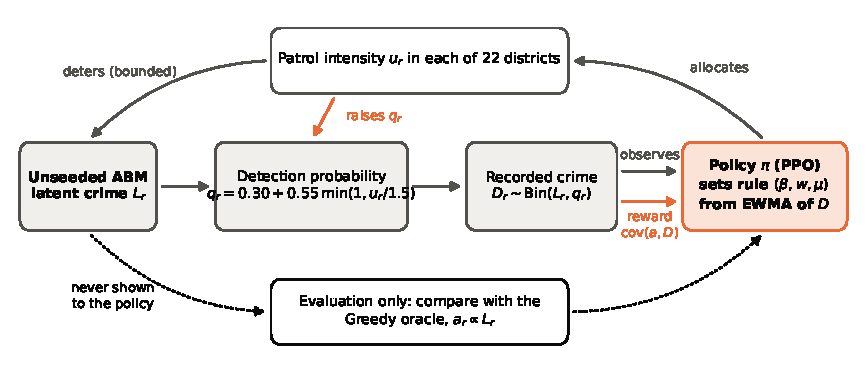
\includegraphics[width=0.82\textwidth]{figures/fig_arch.pdf}
\caption{The closed loop. Latent crime $L_r$ is thinned into recorded crime
$D_r$ with a detection probability that rises with patrol intensity $u_r$. The
policy observes only recorded crime and is rewarded for covering it. Latent
crime is used only for evaluation, through the need-proportional reference.}
\label{fig:arch}
\end{figure*}

We ask:
\begin{itemize}
\item[\textbf{E1}] How far from the need-proportional reference does an RL
allocator trained on recorded crime move enforcement, and what does it cost in
true-crime coverage?
\item[\textbf{E2}] Does the policy contaminate its own objective?
\item[\textbf{E3}] Does the excess fall on disadvantaged districts once their
latent need is controlled for?
\item[\textbf{E4}] Can a penalty remove the excess without overcorrecting?
\item[\textbf{E5}] How much of the excess disappears when patrol no longer
changes detection?
\end{itemize}

\noindent\textbf{Contributions.}
(1)~A closed-loop testbed with known ground truth, in which an RL policy's
observations are contaminated by its own actions, released as a Gymnasium
environment.
(2)~A reference-relative bias measure (paired log-ratio to a need-proportional
allocation, with a hierarchical bootstrap over training and evaluation seeds)
that separates excess concentration from legitimate targeting.
(3)~An attribution of the excess: removing the detection channel (E5), a
$2\times2$ of observation and reward, and a non-RL search over the same rule
class, which locates the bias in the proxy objective rather than in RL itself.
(4)~Evidence that parity penalties overcorrect, and a penalty targeted at the
reference that gets closer to it while raising true-crime coverage.

\section{Related Work}

\textbf{Performative and selectively labelled data.}
Perdomo et al.~\cite{perdomo2020} study predictions that influence the outcomes
they forecast and characterise when repeated retraining converges. Lakkaraju et
al.~\cite{lakkaraju2017} show that when a decision determines which outcomes are
observed, naive evaluation is biased. Our setting combines both: the action
changes which crimes are recorded, and the policy learns from the record.

\textbf{Feedback loops in predictive policing.}
Ensign et al.~\cite{ensign2018} model discovered-incident feedback with P\'olya
urns and give black-box corrections. Lum and Isaac~\cite{lum2016} show the
disparate impact empirically. A simulation study of predictive versus hot-spots
policing in Baltimore~\cite{algorithms2026} finds the predictive system faster
to amplify bias, and FairSense~\cite{fairsense2025} simulates long-term fairness
of ML-enabled systems in general. None places a sequential RL learner in the loop
or evaluates against a known latent process.

\textbf{RL for patrol allocation.}
Repasky et al.~\cite{repasky2024} treat each patrol unit as a Q-learner; the
cooperative-routing model of~\cite{jocv2025} maximises coverage of historical
crime with a decentralised POMDP; and~\cite{ceus2025} uses deep RL to solve a
maximum-coverage design problem with a regional-disparity constraint. All three
optimise coverage of a fixed signal; the policy's actions do not enter its data.

\textbf{Constrained and fair RL; crime ABMs.}
Our penalties follow the constrained-MDP literature~\cite{chow2017,
tessler2019, stooke2020}, and the exposure constraint follows demographic parity
in sequential decisions~\cite{dwork2012, jabbari2017}. Wise and
Cheng~\cite{wise2024} give offender agents RL; we keep offenders rule-based.
Our generator continues data-driven and routine-activity crime
ABMs~\cite{roses2021, palma2025, caresim2023}; the distinguishing choice is the
flat, unseeded risk surface.

\section{The Emergent Crime Simulator}

A $20\times20$ grid overlays Chicago; each cell takes its modal police district,
giving 22 districts as the unit of allocation and fairness. District covariates
are aggregated from the community-area American Community Survey hardship table.
Residential population is treated as uniform across districts, so per-capita
crime is emergent rather than an input. $N=200$ agents have a home district $r$,
employment at the district unemployment rate, and stress
$s_i = s_0 + h_r + \epsilon_i$ with hardship $h_r\in[0,1]$,
$\epsilon_i\sim\mathcal{U}(0,0.2)$ and $s_0=0.2$. They move on routine-activity
schedules (work 9--17, leisure 18--23, home otherwise).

The environmental risk grid starts at a uniform constant, and \emph{no historical
crime coordinates enter it at any point}; it decays and grows with local
occupancy. An agent commits a violent act through an environmental path, when a
smoothed risk combining stress, local risk and a mean-field escalation term
exceeds a threshold, or through an interaction path whose rate rises with nearby
high-stress agents~\cite{roses2021}. One shift is four sub-steps and yields the
latent violent-crime count per district, $L_r$. The vectorised generator passes
the calibration gate of the earlier Mesa model: crime rises with hardship
(by 27\% from low- to high-hardship scenarios), monotonically across
three scenarios, clusters spatially from the flat start, and is higher at night.

\section{Closed-Loop Allocation and Measurement}

\subsection{Action: rule parameters}
The environment keeps an exponentially weighted moving average $\bar D_r$ of
recorded crime (half-life 5 shifts). An action $(\beta, w, \mu)$ gives the
deployment share
\begin{equation}
a_r \;\propto\; (1-\mu)\,
\frac{(\bar D_r/\overline{\bar D})^{\beta}\, e^{\,w\, z_r}}
{\sum_{r'} (\bar D_{r'}/\overline{\bar D})^{\beta}\, e^{\,w\, z_{r'}}}
\;+\; \frac{\mu}{22},
\end{equation}
with $z_r$ the standardised district hardship, $\beta\in[0,4]$ the concentration
on recorded crime, $w\in[-2,2]$ an explicit hardship tilt and $\mu\in[0,1]$ a
uniform mix, plus a floor of $0.005$ per district. The rule always reads
\emph{recorded} crime; giving the policy latent crime changes its observation,
not the rule's input. A PredPol-style heuristic~\cite{ensign2018} is the rule
with $(\beta, w, \mu) = (1, 0, 0)$.

\subsection{Transition and self-contaminated observation}
With patrol intensity $u_r$ relative to a proportional allocation, deterrence
removes $\min(0.68, 0.26\,u_r)$ of latent crime~\cite{weisburd2017}, and the
recorded count is a thinning
\begin{equation}
D_r \sim \mathrm{Binomial}(L_r,\, q_r), \qquad
q_r = 0.30 + 0.55\,\min(1, u_r/1.5).
\end{equation}
The observation kernel $P(D \mid L, u)$ therefore depends on the policy's own
action: this is the contamination. Under uniform patrol $q_r = 0.667$ everywhere.
The policy observes $\bar D$, its last deployment, time of day and static district
covariates, never $L$.

\subsection{Objectives and policies}
With $\mathrm{cov}(a, X) = \sum_r a_r X_r / \sum_r X_r$, the reward is the
recorded coverage $\mathrm{cov}(a, D)$, the operational criterion of predictive
policing. We report it alongside the true-crime coverage $\mathrm{cov}(a, L)$.
The learner is PPO~\cite{schulman2017ppo, sb3} with a two-layer MLP, trained for
400k steps on randomly seeded episodes of 140 shifts. Baselines: Uniform, Random,
PredPol (EWMA), a random-forest hotspot model refit every 15 shifts, and the
\emph{greedy oracle}, $a_r \propto \bar L_r$, which is not deployable. Two
penalised families subtract a cost from the reward each shift:
\begin{align}
\text{parity:}\quad & w\,\delta_t, \\
\text{oracle-targeted:}\quad & w\,\max\!\big(0,\ \ln\delta_t - \ln\delta_{\mathrm{ref}}\big),
\end{align}
where $\delta_t$ is the per-shift disparity defined below and
$\delta_{\mathrm{ref}} = \nORdisp$ is the greedy oracle's mean per-shift
disparity on reference seeds 1000--1009, disjoint from every evaluation seed.

\subsection{Measuring bias relative to need}
Districts are split into hardship quintiles of 4--5 districts. The
\emph{disparity} $\delta$ of an episode is the mean patrol exposure per capita in
the most disadvantaged quintile divided by that in the least disadvantaged. High
hardship districts do have more latent crime, so $\delta>1$ is not by itself a
bias. We take the greedy oracle as a \emph{normative reference} -- patrol in
proportion to need -- and report, for policy $\pi$ on evaluation seed $e$,
\begin{equation}
\Delta_{\pi,e} = \ln\delta_{\pi,e} - \ln\delta_{\mathrm{oracle},e},
\qquad
\times\text{oracle} = \exp\big(\overline{\Delta}\big),
\end{equation}
a geometric-mean ratio paired on the evaluation seed. 95\% confidence intervals
come from a hierarchical bootstrap (4000 replicates) that resamples training
seeds and then evaluation seeds, keeping evaluation seeds paired across policies.
The reference is not an efficiency bound: the best fixed rule for true-crime
coverage beats it (\nBRLlat{} vs \nORlat) at \nBRLx$\times$ its disparity. We
also report the \emph{proxy gap} $\mathrm{cov}(a,D)-\mathrm{cov}(a,L)$ and the
\emph{over-recording ratio}: the recorded-to-latent crime share in the top
hardship quintile divided by the same in the bottom quintile.

\textbf{Evaluation protocol.} The main experiments use 5 training seeds (0--4)
and 30 held-out evaluation seeds (200--229). The $2\times2$ cells and the
oracle-targeted penalty use training seeds 0--2. E5 uses 3 training seeds and 20
evaluation seeds (300--319), each setting against its own oracle. Pairwise
comparisons use the same bootstrap and two-sided bootstrap $p$-values,
Holm-adjusted over all \nNContrasts{} pre-specified contrasts
(Table~\ref{tab:contrasts}).

\section{Results}

\begin{table*}[t]
\caption{E1/E4. Disparity relative to the greedy oracle (geometric mean with 95\%
hierarchical-bootstrap CI), raw disparity, coverage of true and recorded crime,
proxy gap and over-recording ratio. Eval seeds 200--229; ``Seeds'' = training
seeds.}
\label{tab:e1}
\centering
\begin{tabular}{lccccccc}
\toprule
Policy & Seeds & $\times$ oracle [95\% CI] & Disparity & True cov. & Rec.\ cov. &
Proxy gap & Q5/Q1 over-rec. \\
\midrule
Greedy oracle & -- & 1 (ref.) & 2.78 & 0.0537 & 0.0567 & 0.0030 & 1.58 \\
Uniform & -- & 0.36 [0.35, 0.37] & 1.00 & 0.0455 & 0.0455 & 0.0000 & 1.00 \\
Random & -- & 0.36 [0.35, 0.37] & 1.00 & 0.0413 & 0.0472 & 0.0058 & 1.01 \\
PredPol (EWMA) & -- & 1.41 [1.39, 1.42] & 3.92 & 0.0548 & 0.0595 & 0.0047 & 1.75 \\
Random forest & -- & 1.36 [1.33, 1.39] & 3.78 & 0.0547 & 0.0591 & 0.0044 & 1.68 \\
\midrule
Best fixed rule, true cov. & -- & 2.24 [2.19, 2.28] & 6.26 & 0.0552 & 0.0626 & 0.0074 & 1.96 \\
Best fixed rule, recorded cov. & -- & 13.04 [12.70, 13.39] & 36.26 & 0.0475 & 0.0746 & 0.0271 & 2.46 \\
\midrule
PPO (naive) & 5 & 3.91 [2.98, 5.08] & 12.32 & 0.0477 & 0.0672 & 0.0196 & 1.89 \\
PPO, sees + rewarded on true crime & 5 & 1.22 [1.11, 1.35] & 3.50 & 0.0490 & 0.0571 & 0.0081 & 1.42 \\
\midrule
Parity penalty 0.02 & 5 & 0.66 [0.57, 0.75] & 1.88 & 0.0481 & 0.0532 & 0.0051 & 1.20 \\
Parity penalty 0.06 & 5 & 0.34 [0.33, 0.35] & 0.94 & 0.0449 & 0.0483 & 0.0034 & 0.97 \\
Parity penalty 0.15 & 5 & 0.25 [0.24, 0.27] & 0.71 & 0.0427 & 0.0460 & 0.0033 & 0.87 \\
Parity penalty 0.4 & 5 & 0.11 [0.09, 0.12] & 0.31 & 0.0339 & 0.0381 & 0.0042 & 0.67 \\
\midrule
Oracle-targeted penalty 0.05 & 3 & 2.98 [2.57, 3.53] & 9.46 & 0.0482 & 0.0654 & 0.0172 & 1.80 \\
Oracle-targeted penalty 0.15 & 3 & 0.76 [0.69, 0.85] & 2.12 & 0.0490 & 0.0534 & 0.0044 & 1.29 \\
Oracle-targeted penalty 0.5 & 3 & 0.53 [0.45, 0.72] & 1.52 & 0.0479 & 0.0506 & 0.0026 & 1.16 \\

\bottomrule
\end{tabular}
\end{table*}

\subsection{E1: excess concentration at a coverage cost}
Naive PPO's disparity is \nPPOx$\times$ the oracle's (95\% CI
\nPPOxLo--\nPPOxHi; Table~\ref{tab:e1}, Fig.~\ref{fig:e1}) and
\nPPOvsEWMA$\times$ the PredPol heuristic's. The five training seeds range from
\nPPOseedMin$\times$ to \nPPOseedMax$\times$; this instability is part of the
result and is carried by the interval. PPO has the second-highest recorded
coverage of any policy (\nPPOrec, against \nEWMArec{} for PredPol), but its
true-crime coverage (\nPPOlat) is below the oracle's (\nORlat), PredPol's
(\nEWMAlat) and every hotspot baseline. The rule it learns
(Table~\ref{tab:rules}) concentrates sharply on recorded crime
($\beta\approx\nPPObeta$), adds an explicit tilt toward high-hardship districts
($w\approx\nPPOw$) and almost no uniform mix ($\mu\approx\nPPOmu$).

\begin{figure*}[t]\centering
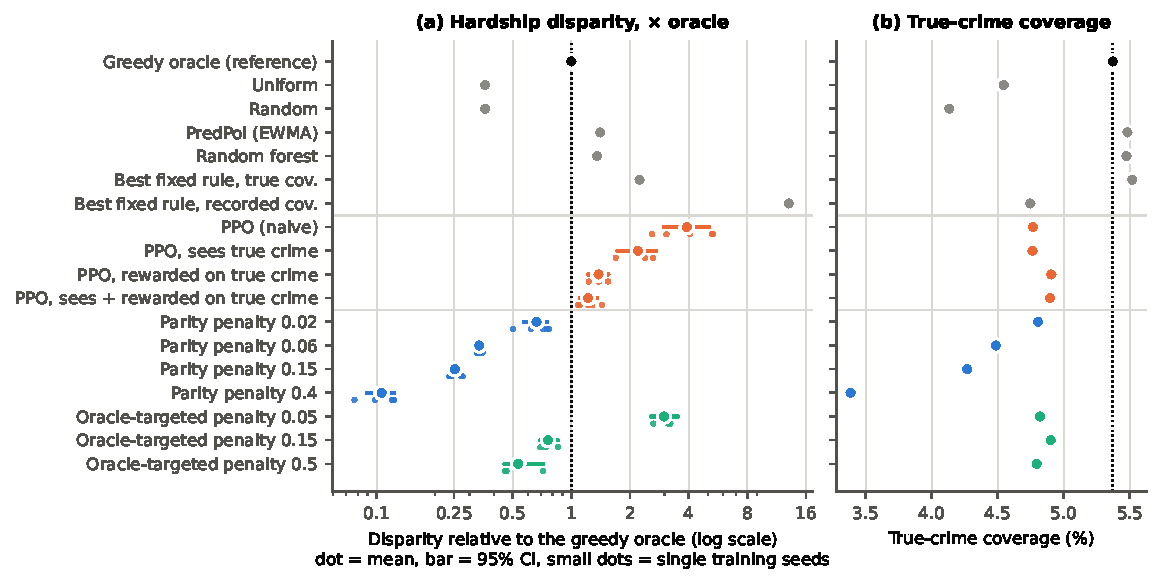
\includegraphics[width=0.9\textwidth]{figures/fig_e1_disparity.pdf}
\caption{E1/E4. (a) Disparity relative to the greedy oracle; 1 = need-proportional
patrol. (b) Coverage of true crime; the dotted line is the oracle.}
\label{fig:e1}
\end{figure*}

\textbf{Is the bias specific to RL?} We searched the same rule class without RL:
192 fixed $(\beta, w, \mu)$ settings scored on seeds 1000--1002, then re-evaluated
on the evaluation seeds. The fixed rule that maximises PPO's own reward reaches a
higher recorded coverage (\nBRRrec{} vs \nPPOrec), so PPO is under-optimised, and
it is far more skewed (\nBRRx$\times$ the oracle) with a maximal hardship tilt.
Pushing harder on the recorded-crime objective produces more disparity, not less:
the bias is a property of the objective, which RL partially optimises.

\begin{table}[t]
\caption{Rule parameters. RL rows: mean action over 5 eval episodes per training
seed, averaged over seeds.}
\label{tab:rules}
\centering
\begin{tabular}{lccc}
\toprule
Policy & $\beta$ & $w$ & $\mu$ \\
\midrule
PPO (naive) & 3.10 & $+1.28$ & 0.14 \\
PPO, sees true crime & 3.05 & $+0.80$ & 0.29 \\
PPO, rewarded on true crime & 2.31 & $+0.81$ & 0.48 \\
PPO, sees + rewarded on true crime & 2.55 & $+0.57$ & 0.51 \\
Parity penalty 0.02 & 2.76 & $+0.10$ & 0.57 \\
Parity penalty 0.4 & 0.67 & $-1.57$ & 0.51 \\
Oracle-targeted penalty 0.15 & 2.41 & $+0.36$ & 0.59 \\
\midrule
Best fixed rule, recorded cov. & 4.00 & $+2.00$ & 0.00 \\
Best fixed rule, true cov. & 1.50 & $+0.00$ & 0.00 \\
PredPol (EWMA), equivalent rule & 1.00 & $+0.00$ & 0.00 \\

\bottomrule
\end{tabular}
\end{table}

\subsection{E2: the policy inflates its own objective}
Naive PPO's proxy gap is \nPPOgap{} -- recorded coverage overstates true
coverage by about two percentage points -- against \nEWMAgap{} for PredPol and
\nORgap{} for the oracle (Table~\ref{tab:e1}). The gap opens in the first shifts
and widens over the episode (Fig.~\ref{fig:e2}a). The records it learns from are
tilted: the top hardship quintile is over-recorded relative to the bottom one by
a factor of \nPPOrd, against \nORrd{} for the oracle. We also computed a
self-induced signal (the partial correlation between last shift's patrol and this
shift's over-recording). It is high for every targeted policy (PPO \nPPOsis,
oracle \nORsis, PredPol \nEWMAsis), so it measures the strength of the detection
channel rather than a policy-specific loop, and we do not use it as evidence. We
likewise drop the ``runaway index'' of our earlier draft: a static allocation
with no feedback scores 1.0 on it.

\begin{figure*}[t]\centering
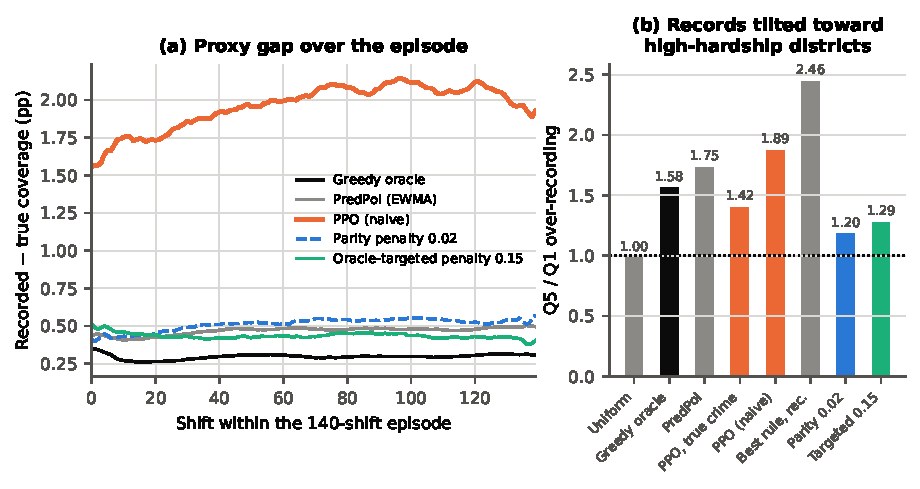
\includegraphics[width=0.82\textwidth]{figures/fig_e2_contamination.pdf}
\caption{E2. (a) Recorded minus true coverage over the episode, mean over
evaluation episodes. (b) Over-recording of the top hardship quintile relative to
the bottom one; 1 = records are not tilted.}
\label{fig:e2}
\end{figure*}

\subsection{E3: excess on disadvantaged districts, beyond need}
For every (episode, shift, district) after a 30\% burn-in we regress the
\emph{allocation residual} $a_r - n_r$ on standardised hardship, need and
poverty, where the need $n_r$ is the district's long-run latent-crime share under
uniform patrol on the same evaluation seeds. Standard errors are clustered on
episode, and a seed-level bootstrap resamples per-training-seed coefficients
(Table~\ref{tab:e3}). The coefficient is descriptive, not causal. Naive PPO's
hardship coefficient is $+\nPPOcoef\times10^{-3}$ per standard deviation
($t=\nPPOt$; seed-level 95\% CI \nPPOcoefLo--\nPPOcoefHi; positive in
\nPPOseedsPos{} seeds), while the oracle and the hotspot baselines show none.
Fig.~\ref{fig:e3} shows the shape: PPO gives the most disadvantaged quintile
\nPPOqfive{} percentage points of patrol share beyond need and takes it from the
middle quintiles (down to \nPPOqtwothree{} points). The proxy-maximising fixed
rule has the same sign and is larger ($+\nBRRcoef\times10^{-3}$). This is
about a quarter of the effect our earlier draft reported ($+0.017$ with
$p<10^{-300}$), which controlled only for the current shift's latent share and
treated region-shifts as independent.

\begin{table}[t]
\caption{E3. Hardship coefficient on the allocation residual
($\times10^{-3}$ per s.d.), episode-clustered $t$, seed-level bootstrap CI and
the number of training seeds with a positive coefficient.}
\label{tab:e3}
\centering
\setlength{\tabcolsep}{4pt}
\begin{tabular}{lcccc}
\toprule
Policy & Coef. & $t$ & Seed CI & $>0$ \\
\midrule
Greedy oracle & $-0.7$ & -1.3 & -- & -- \\
Uniform & \multicolumn{4}{c}{constant allocation; not estimable} \\
PredPol (EWMA) & $-0.5$ & -0.8 & -- & -- \\
Random forest & $+0.7$ & 1.4 & -- & -- \\
Best fixed rule, recorded cov. & $+10.3$ & 8.7 & -- & -- \\
PPO (naive) & $+3.8$ & 7.8 & [2.0, 5.6] & 5/5 \\
PPO, sees + rewarded on true crime & $+1.4$ & 4.4 & [0.7, 2.2] & 5/5 \\
PPO, sees true crime & $-0.2$ & -0.3 & [-4.1, 3.2] & 2/3 \\
PPO, rewarded on true crime & $+2.3$ & 6.0 & [1.5, 2.9] & 3/3 \\
Parity penalty 0.02 & $-12.0$ & -19.8 & [-16.1, -8.3] & 0/5 \\
Parity penalty 0.4 & $-43.1$ & -52.4 & [-47.3, -38.9] & 0/5 \\
Oracle-targeted penalty 0.15 & $-5.0$ & -10.9 & [-8.4, -1.7] & 0/3 \\

\bottomrule
\end{tabular}
\end{table}

\begin{figure}[t]\centering
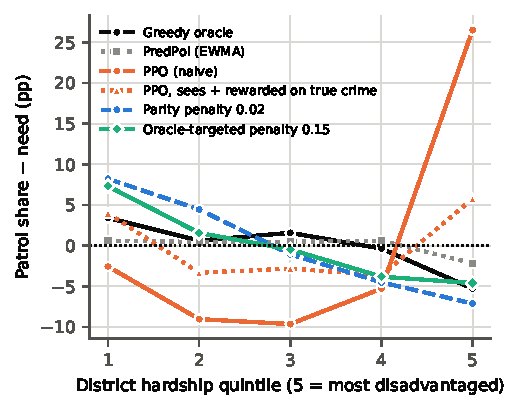
\includegraphics[width=\linewidth]{figures/fig_e3_need_residual.pdf}
\caption{E3. Patrol share minus latent need, summed within each hardship
quintile (after a 30\% burn-in).}
\label{fig:e3}
\end{figure}

\subsection{Attribution: reward or observation?}
Table~\ref{tab:attr} crosses what PPO observes with what it is rewarded on.
Rewarding true-crime coverage while still observing only recorded crime cuts the
excess from \nAttRecRec$\times$ to \nAttRecLat$\times$; letting the policy observe
true crime while still rewarding recorded coverage cuts it only to
\nAttLatRec$\times$. Both together give \nAttLatLat$\times$, still above the
oracle because the rule reads recorded crime. The reward is the larger lever.

\begin{table}[t]
\caption{$2\times2$ attribution, $\times$ oracle [95\% CI], training seeds
0--2.}
\label{tab:attr}
\centering
\setlength{\tabcolsep}{4pt}
\begin{tabular}{lcc}
\toprule
& \multicolumn{2}{c}{Rewarded on} \\
Observes & recorded crime & true crime \\
\midrule
Recorded crime only & 4.85 [3.97, 5.73] & 1.38 [1.22, 1.55] \\
Recorded + true crime & 2.20 [1.72, 2.72] & 1.20 [1.05, 1.42] \\

\bottomrule
\end{tabular}
\end{table}

\subsection{E4: penalties overcorrect; a targeted penalty does better}
A penalty on raw disparity pushes $\delta$ toward 0, not toward need. Every
parity weight lands \emph{below} the oracle -- \nPtwox$\times$ at the lightest
($w=0.02$) and \nPfourx$\times$ at the heaviest -- and E3 coefficients turn
negative (\nPtwoCoef$\times10^{-3}$ at $w=0.02$): disadvantaged districts end up
under-patrolled relative to need, and true-crime coverage falls to \nPfourlat{}
at $w=0.4$. The oracle-targeted penalty charges only for disparity above the
reference. At $w=0.15$ it reaches \nRonefivex$\times$ the oracle (95\% CI
\nRonefiveLo--\nRonefiveHi), the closest of any learned policy, and raises
true-crime coverage above naive PPO's (\nRonefivelat{} vs \nPPOlat; Holm
$p=\nRonefiveLatP$). It does not hit the target exactly: $w=0.05$ is too weak
(\nRfivex$\times$) and $w=0.5$ lands at \nRhalfx$\times$ (Fig.~\ref{fig:e4}).

\begin{figure}[t]\centering
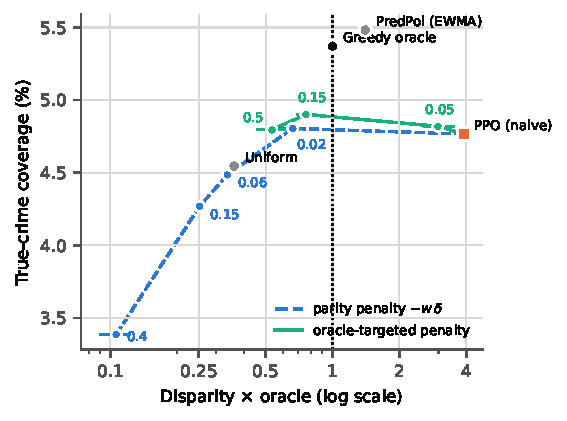
\includegraphics[width=\linewidth]{figures/fig_e4_frontier.pdf}
\caption{E4. True-crime coverage against disparity relative to the oracle for the
two penalty families (labels = weight $w$; bars = 95\% CI).}
\label{fig:e4}
\end{figure}

\subsection{E5: removing the detection channel}
We retrain PPO and the parity-penalised agent ($w=0.06$) in two settings where
patrol no longer changes detection, each scored against its own oracle
(Table~\ref{tab:e5}, Fig.~\ref{fig:e5}). \emph{Perfect observation} sets $q_r=1$:
it removes the action-dependence but also raises the volume of recorded crime and
makes the reward equal to true coverage. \emph{Constant detection} sets
$q_r=0.667$ for every district, the uniform-patrol rate, so the volume of data is
unchanged and only the dependence on patrol is removed. PPO's excess drops from
\nEfiveBase$\times$ (\nEfiveBaseLo--\nEfiveBaseHi) to \nEfivePerf$\times$ and
\nEfiveConst$\times$ (\nEfiveConstLo--\nEfiveConstHi) respectively, and
over-recording drops to 1. The constant-detection control shows the reduction is
due to the detection channel, not to more data. A residual of about 1.5$\times$
remains without contamination, which we attribute to the policy's partial
optimisation of a concentrating rule. The parity-penalised agent sits at
\nEfiveFairMin--\nEfiveFairMax$\times$ in every setting. This is
mechanism-isolating evidence within the simulator's structural equations, not
proof of a causal effect in real policing.

\begin{table}[t]
\caption{E5. Oracle disparity and $\times$ own-setting oracle [95\% CI] for
naive and parity-penalised PPO, and PPO's over-recording ratio. 3 training seeds,
eval seeds 300--319.}
\label{tab:e5}
\centering
\setlength{\tabcolsep}{3pt}
\begin{tabular}{lcccc}
\toprule
Setting & Oracle & PPO & Penalised & Over-rec. \\
\midrule
Base (patrol raises detection) & 2.82 & 4.92 [4.05, 5.92] & 0.33 [0.32, 0.34] & 2.01 \\
Perfect observation & 2.82 & 1.65 [1.51, 1.86] & 0.36 [0.34, 0.37] & 1.00 \\
Constant detection, $q=0.667$ & 2.82 & 1.46 [1.36, 1.59] & 0.35 [0.34, 0.37] & 1.00 \\

\bottomrule
\end{tabular}
\end{table}

\begin{figure}[t]\centering
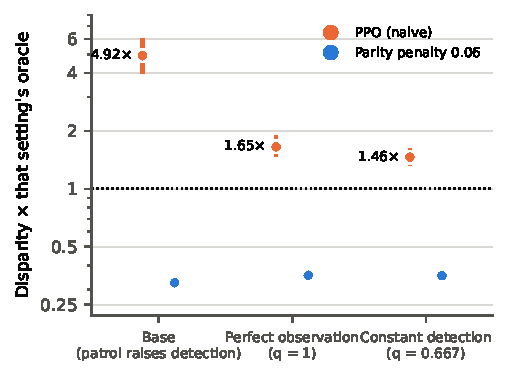
\includegraphics[width=\linewidth]{figures/fig_e5_interventions.pdf}
\caption{E5. Disparity relative to each setting's own greedy oracle (bars = 95\%
CI).}
\label{fig:e5}
\end{figure}

\begin{table*}[t]
\caption{Pre-specified paired contrasts. For disparity, the ratio of geometric
means; for coverage, the difference in percentage points. Two-sided bootstrap
$p$-values, Holm-adjusted over all \nNContrasts{} rows.}
\label{tab:contrasts}
\centering
\begin{tabular}{llccc}
\toprule
Contrast & Metric & Estimate & 95\% CI & $p_{\mathrm{Holm}}$ \\
\midrule
PPO (naive) vs Greedy oracle & disparity & 3.91$\times$ & [2.98, 5.10] & $<0.005$ \\
PPO (naive) vs PredPol (EWMA) & disparity & 2.78$\times$ & [2.12, 3.63] & $<0.005$ \\
PPO (naive) vs Random forest & disparity & 2.88$\times$ & [2.20, 3.77] & $<0.005$ \\
PPO (naive) vs Best fixed rule, recorded cov. & disparity & 0.30$\times$ & [0.23, 0.39] & $<0.005$ \\
PPO, sees true crime vs PPO (naive) & disparity & 0.56$\times$ & [0.40, 0.79] & $<0.005$ \\
PPO, rewarded on true crime vs PPO (naive) & disparity & 0.35$\times$ & [0.27, 0.47] & $<0.005$ \\
PPO, sees + rewarded on true crime vs PPO (naive) & disparity & 0.31$\times$ & [0.24, 0.41] & $<0.005$ \\
PPO, sees + rewarded on true crime vs Greedy oracle & disparity & 1.22$\times$ & [1.10, 1.36] & $<0.005$ \\
PPO (naive) vs Greedy oracle & true cov. & $-0.60$ pp & [-0.66, -0.55] & $<0.005$ \\
PPO (naive) vs Uniform & true cov. & $+0.22$ pp & [+0.14, +0.30] & $<0.005$ \\
PPO (naive) vs Best fixed rule, recorded cov. & recorded cov. & $-0.74$ pp & [-0.93, -0.56] & $<0.005$ \\
Oracle-targeted penalty 0.05 vs Greedy oracle & disparity & 2.98$\times$ & [2.56, 3.54] & $<0.005$ \\
Oracle-targeted penalty 0.15 vs Greedy oracle & disparity & 0.76$\times$ & [0.69, 0.85] & $<0.005$ \\
Oracle-targeted penalty 0.5 vs Greedy oracle & disparity & 0.53$\times$ & [0.45, 0.71] & $<0.005$ \\
Oracle-targeted penalty 0.05 vs PPO (naive) & true cov. & $+0.05$ pp & [+0.00, +0.11] & 0.099 \\
Oracle-targeted penalty 0.15 vs PPO (naive) & true cov. & $+0.13$ pp & [+0.05, +0.22] & $<0.005$ \\
Oracle-targeted penalty 0.5 vs PPO (naive) & true cov. & $+0.03$ pp & [-0.11, +0.20] & 0.726 \\
E5 PPO, perfect obs. vs E5 PPO, base & disparity & 0.34$\times$ & [0.29, 0.41] & $<0.005$ \\
E5 PPO, constant detection vs E5 PPO, base & disparity & 0.30$\times$ & [0.26, 0.36] & $<0.005$ \\

\bottomrule
\end{tabular}
\end{table*}

\section{Discussion}

The naive policy is not failing at its task: given a reward for covering recorded
crime, concentrating on recorded hotspots is the right answer, and a fixed rule
that does so harder is more skewed still. The problem is that the recorded-crime
objective and the social objective -- cover real crime, in proportion to need --
diverge once the allocator can change the record. The divergence lands on the
most disadvantaged districts and is visible only against ground truth. Two
practical readings follow. An allocator that trains on discovered incidents
should be scored against an estimate of latent crime, because its own dashboard
(recorded coverage) rewards the distortion. And an equity constraint should be
referenced to need rather than to parity; parity penalties under-patrol the
districts with the most crime.

\textbf{Limitations.}
(1)~The claims concern a simulated world with parametric deterrence and detection
that are not calibrated to an external estimate of reporting rates.
(2)~Quintiles of 22 districts hold only 4--5 districts each.
(3)~Training is unstable across seeds (\nPPOseedMin--\nPPOseedMax$\times$ for
naive PPO); we report the spread and carry it in every interval, and E5 rests on
3 training seeds.
(4)~PPO acts through a three-parameter rule and is under-optimised within it; a
richer action space could behave differently.
(5)~Residential population is uniform across districts.
(6)~The reference is normative, not optimal: need-proportional patrol is not the
coverage-maximising allocation.
(7)~Offenders do not adapt to patrol.

\section{Conclusion}
In a crime simulator whose latent process is known, an RL allocator rewarded for
covering recorded crime concentrates patrol \nPPOx$\times$ beyond a
need-proportional reference, covers less true crime than simple heuristics, and
over-patrols disadvantaged districts beyond their need. Removing the
patrol-dependence of detection removes most of the excess, the reward is a larger
lever than the observation, and a penalty targeted at need rather than parity
gets closest to the reference. The same pattern -- a learner optimising a signal
it contaminates -- applies wherever actions decide what gets observed.

\section*{Acknowledgment}
We thank PES University and the Department of Computer Science and Engineering
(AI \& ML). This work was carried out as Capstone Project Phase 2 (UE23AM320B).

\bibliographystyle{IEEEtran}
\bibliography{refs}

\end{document}
